\documentclass{article}
\usepackage[utf8]{inputenc}


\begin{document}

\begin{center}
\caption\textbf{HERRAMIENTAS DE BUSINESS ANALITYCS}
\end{center}
\\
\\
Toda empresa necesita un plan de negocio. Muchos emprendedores caen en la tentación de poner en marcha su negocio sin analizar nada previamente y se limitan a cruzar los dedos esperando que salga bien. Y podría ser que sí, pero lo más probable es que no.\\
Lo ideal es llevar a cabo un análisis previo pormenorizado del sector y el mercado en el que pensamos adentrarnos. Hay numerosas herramientas de análisis estratégico gratuitas que nos pueden servir para para identificar qué distingue nuestra marca del resto y elaborar un buen plan de negocio para nuestra futura empresa. Estas son algunas de ellas.  
\\
\begin{itemize}
\item Análisis PEST
\\Con esta herramienta de análisis estratégico podremos analizar el entorno en el que queremos crear o establecer nuestra empresa, negocio o proyecto. Nos permite identificar posibles cambios de escenario en nuestro sector o en la región para detectar y aprovechar posibles oportunidades de crecimiento. El nombre es un acrónimo de cuatro factores:

Políticos: estabilidad política, la posibilidad de un cambio de gobierno que de lugar a cambios en las políticas fiscales o en materia de subvenciones, posibles cambios en los tratados comerciales, existencia o no de grupos de presión.
Económicos: economía en crecimiento o en recesión, tendencia del consumo, situación de confianza o de inestabilidad, los tipos de cambio, el nivel de inflacción…
Socioculturales: hábitos sociales, cambios en los gustos o en las modas de la gente, formas de comunicación habituales, demografía, salud, valores.
Tecnológicos: tecnología actual, posibles avances, desarrollos en marcha, conocimientos, inversión en I+D, información.
Debemos analizar en qué medida cada uno de estos factores macroambientales podría influir positiva o negativamente en nuestra empresa.  
		\begin{center}
		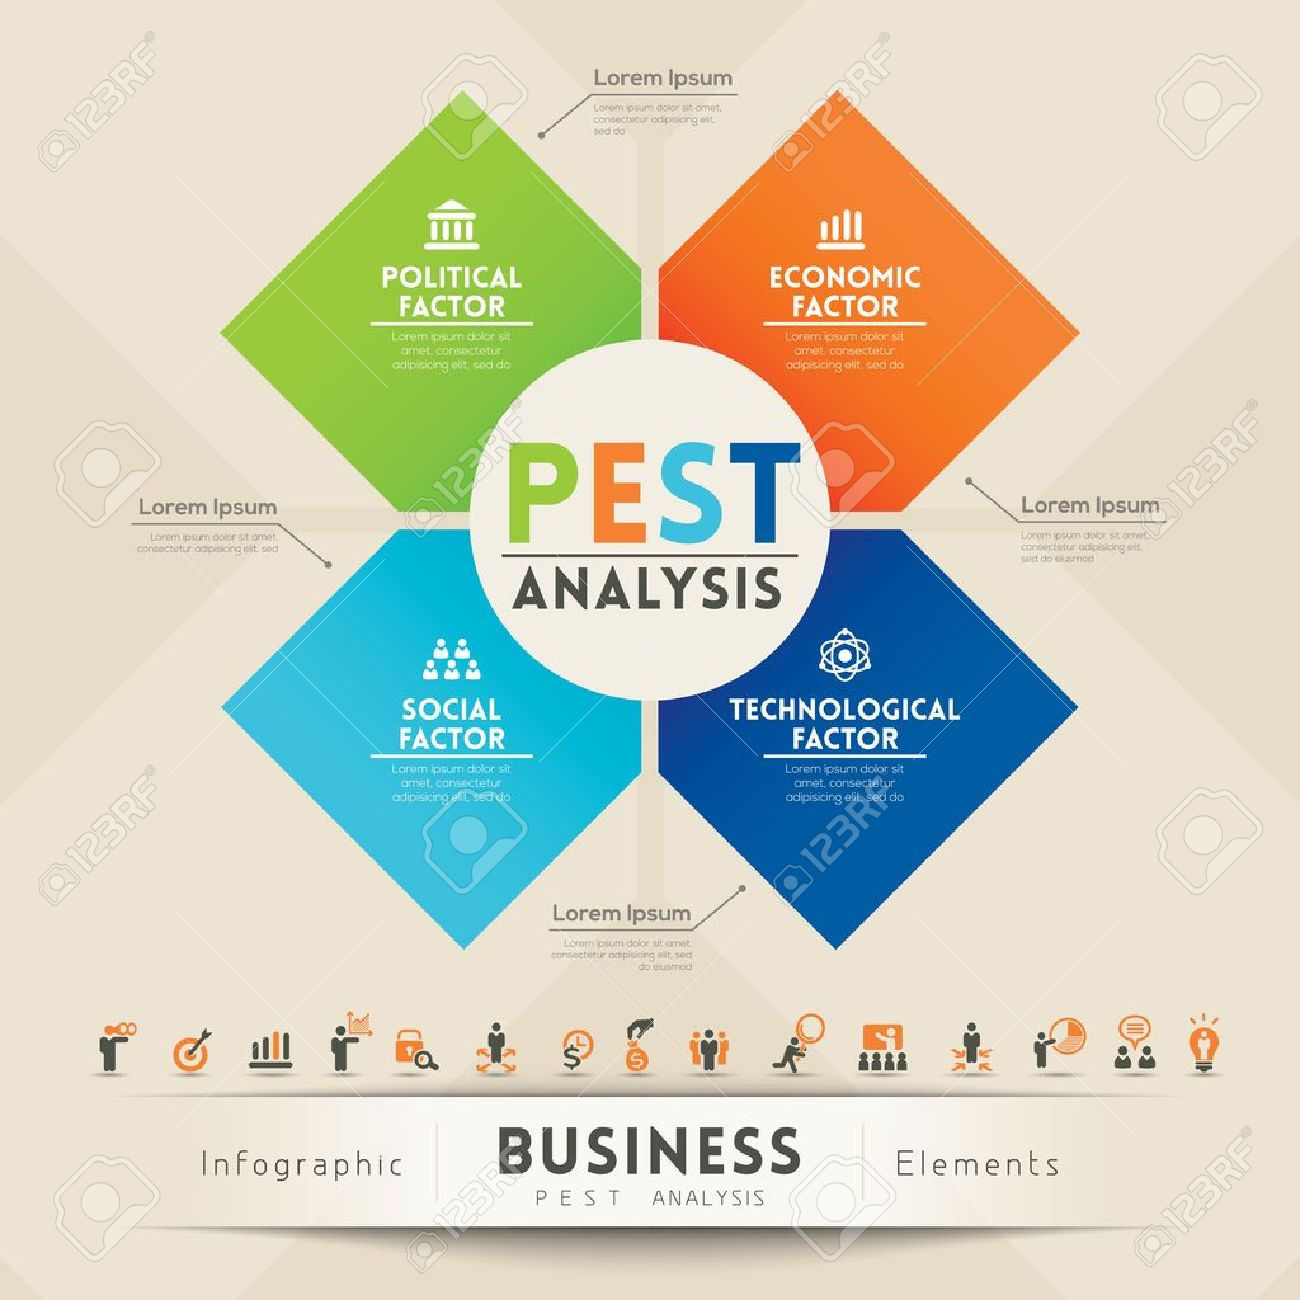
\includegraphics[width=15cm]{./Imagenes/Imagen1}
		\end{center}

	\end{itemize} 
	
	\begin{itemize}
\item Análisis PESTEL
\\Es una variación del anterior que añade dos factores más a los cuatro del análisis PEST. Además de tener en cuenta los factores políticos, económicos, sociales y tecnológicos, se analizarán también los factores:

Ecológicos: por ejemplo, el cambio climático puede tener consecuencias en diversos sectores como el turístico o el de las aseguradoras. Las leyes de protección medioambiental o las regulaciones en materia de gestión de residuos o de energías también pueden influir en una empresa.
Legales: leyes contra la discriminación, leyes de defensa del consumidor, leyes antimonopolio, licencias, legislación laboral, leyes de protección de la salud, sectores con una protección especial.
		\begin{center}
		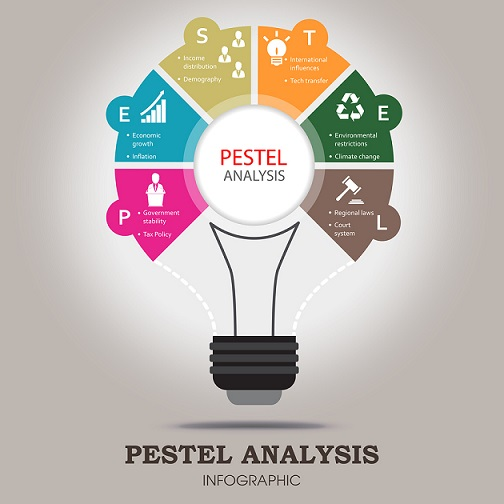
\includegraphics[width=15cm]{./Imagenes/Imagen2}
		\end{center}
	\end{itemize} 

\end{document}
